% Provenance (never printed): old premiere S material on the lithosphere and the
% asthenosphere (chemical and mechanical layers, the low-velocity zone, the
% geotherm, isostasy); see sources/book2/PROVENANCE.md. S speeds from
% figdata/grade-11/prem_profiles.py (part upper), the geotherm and the solidus
% from geotherm_solidus.py, the elevations from hypsometry.py (ETOPO1).
% Glacial rebound belongs to g12; lithostatic pressure (term) to g12.
\chapter{Litosfera e astenosfera}\label{ch:g11:lithosphere-asthenosphere}

Nove décimos de um iceberg ficam debaixo da água: o gelo flutua porque é um
pouco menos denso que o mar, e afunda na água até que a água que ele
desloca pese tanto quanto o iceberg inteiro. As cadeias de montanhas se
comportam mais ou menos da mesma maneira. Sob as mais altas delas, a crosta
é quase duas vezes mais espessa que o normal, e a maior parte dessa crosta a
mais fica escondida por baixo, como o gelo sob a linha da água. Mas um
iceberg flutua num líquido, e o manto sob uma cadeia de montanhas é rocha
sólida. Este capítulo mostra como um sólido pode se comportar como um
fluido sobre o qual flutua a camada externa da Terra, e o que é essa camada.
% ledger: usgs:ice-density, karplus:tibet-moho, cm95:crust

\begin{recall}
A Terra tem uma crosta, um manto e um núcleo (Livro 1, 6º ano). O \omterm{def:g11:seismic-structure:moho}{Moho}, na
base da crosta, fica em média a cerca de \qty{41}{km} de profundidade sob os
continentes e alguns quilômetros abaixo do fundo do oceano; as velocidades
sísmicas e as densidades são conhecidas em cada profundidade a partir de um
\omterm{def:g11:seismic-structure:reference-model}{modelo de referência da Terra} (\cref{ch:g11:seismic-structure}). A rocha
fica mais quente com a profundidade, cerca de 25 a \qty{30}{\celsius} por
quilômetro perto da superfície (Livro 1, 6º ano). Um corpo que flutua num
líquido desloca um peso de líquido igual ao seu próprio peso, e a pressão na
base de uma coluna de material é o peso da coluna dividido pela sua área
(os livros de física).
\end{recall}
% ledger: cm95:crust, usgs:crust-thickness, usgs:gradient-29 (Book 1 rows)

\begin{omfigure}
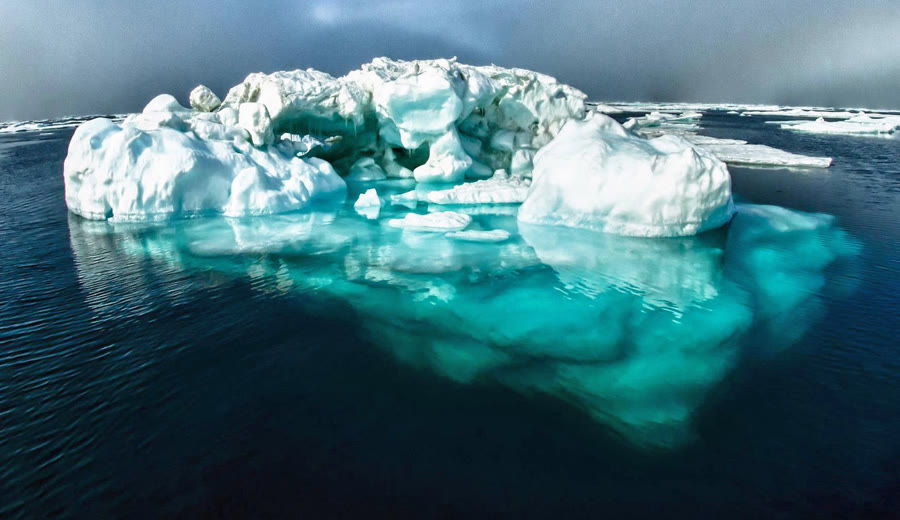
\includegraphics[width=0.66\linewidth]{images/book2/g11-noaa-iceberg.jpg}

{\small Um iceberg visto logo acima da água: o gelo sob a superfície, que
aparece através do mar transparente, é muito maior que a parte no ar.
Fotografia: NOAA (domínio público).}
\end{omfigure}
% ledger: photo:g11-iceberg

\section{Duas maneiras de dividir a Terra em camadas}

A crosta, o manto e o núcleo são camadas de \emph{materiais} diferentes: a
crosta é feita de rochas ricas em silício, alumínio e oxigênio, o manto de
uma rocha mais densa, o núcleo de metal. Mas a parte externa da Terra também
pode ser dividida segundo o modo como a sua rocha se \emph{comporta} quando
forças agem sobre ela durante muito tempo.

\begin{definition}[Litosfera; astenosfera]\label{def:g11:lithosphere-asthenosphere:lithosphere}
A \emph{litosfera}\index{litosfera} é a camada externa rígida da Terra: a
crosta e a parte mais alta e mais fria do manto, que juntas se partem nas
placas tectônicas e não escoam. A \emph{astenosfera}\index{astenosfera} é a
camada do manto abaixo da litosfera, mais quente e mais fraca, que escoa
lentamente ao longo de grandes intervalos de tempo, como uma pasta muito
dura.
\end{definition}

A fronteira entre as duas fica a cerca de 70 a \qty{100}{km} de
profundidade sob os oceanos e a maioria dos continentes, e mais fundo sob as
partes mais antigas dos continentes; através dos Estados Unidos, por
exemplo, a \omterm{def:g11:lithosphere-asthenosphere:lithosphere}{litosfera} vai de cerca de \qty{40}{km} de espessura no oeste a
mais de \qty{200}{km} no meio do continente. A base da \omterm{def:g11:lithosphere-asthenosphere:lithosphere}{litosfera} não é o
\omterm{def:g11:seismic-structure:moho}{Moho}: a maior parte da \omterm{def:g11:lithosphere-asthenosphere:lithosphere}{litosfera} é rocha do manto.
% ledger: rs09:lab, fischer:lab, porter:lab, usgs:lithosphere-80km (Book 1 row)

\begin{omfigure}
\begin{tikzpicture}[x=1cm, y=-0.0125cm, font=\footnotesize]
% depths to scale: crust 41 km (cm95:crust), lithosphere 100 km (rs09:lab), 0-400 km
  \shade[top color=omLithPeridotite!70, bottom color=omLithPeridotite!25] (5,100) rectangle (8,400);
  \fill[omLithGranite!55] (0,0) rectangle (3,41);
  \fill[omLithPeridotite!55] (0,41) rectangle (3,400);
  \fill[black!25] (5,0) rectangle (8,100);
  \draw (0,0) rectangle (3,400);
  \draw (5,0) -- (5,400) (8,0) -- (8,400) (5,0) -- (8,0);
  \draw[line width=0.8pt] (0,41) -- (3,41);
  \draw[line width=0.8pt, densely dashed] (5,100) -- (8,100);
  \draw[densely dotted, black!60] (3,41) -- (5,41);
  \node at (1.5,20) {crosta};
  \node[align=center] at (1.5,220) {manto};
  \node[align=center] at (6.5,50) {litosfera\\rígida};
  \node[align=center] at (6.5,180) {astenosfera\\fraca,\\escoa devagar};
  \node[align=center, text=black!70] at (6.5,340) {manto mais\\profundo};
  \node[anchor=south, font=\small] at (1.5,0) {pelo material};
  \node[anchor=south, font=\small] at (6.5,0) {pelo comportamento};
  \foreach \d in {0,100,200,300,400} {\draw (-0.1,\d) -- (0,\d); \node[anchor=east] at (-0.1,\d) {\d};}
  \node[anchor=east, rotate=90, anchor=south] at (-0.9,200) {profundidade (\unit{km})};
  \node[anchor=south, font=\scriptsize, align=center] at (4,41) {Moho\\(\qty{41}{km})};
  \node[anchor=west, align=left] at (8.15,100) {base da\\litosfera\\(cerca de \qty{100}{km})};
\end{tikzpicture}

{\small Os \qty{400}{km} superiores da Terra sob um continente, em escala.
À esquerda: as camadas pelo material. À direita: as camadas pelo
comportamento. A \omterm{def:g11:lithosphere-asthenosphere:lithosphere}{litosfera} rígida contém a crosta inteira e o topo do
manto; a \omterm{def:g11:lithosphere-asthenosphere:lithosphere}{astenosfera} não tem um limite inferior nítido.}
\end{omfigure}

\section{A zona de baixa velocidade}

As ondas sísmicas mostram a \omterm{def:g11:lithosphere-asthenosphere:lithosphere}{astenosfera}. Quase em toda parte na Terra, as
velocidades sísmicas aumentam com a profundidade, porque a rocha está cada
vez mais comprimida. Sob a \omterm{def:g11:lithosphere-asthenosphere:lithosphere}{litosfera}, acontece o contrário.

\begin{definition}[Zona de baixa velocidade]\label{def:g11:lithosphere-asthenosphere:lvz}
A \emph{zona de baixa velocidade}\index{zona de baixa velocidade} é a camada
do manto superior, abaixo da \omterm{def:g11:lithosphere-asthenosphere:lithosphere}{litosfera}, na qual as ondas sísmicas se
propagam mais devagar que na rocha acima e abaixo dela.
\end{definition}

No \omterm{def:g11:seismic-structure:reference-model}{modelo de referência da Terra}, a velocidade S cai lentamente do \omterm{def:g11:seismic-structure:moho}{Moho} até
\qty{220}{km}, e depois salta para cima. Os estudos sísmicos no mundo inteiro
encontram uma queda nítida de velocidade em algum ponto entre 70 e
\qty{100}{km}: o topo da \omterm{def:g11:lithosphere-asthenosphere:lithosphere}{astenosfera}. A rocha ali é quente o bastante para
estar perto da fusão, e pode conter uma quantidade muito pequena de material
fundido; ela também pode conter mais água que a rocha de cima. Uma rocha
perto da fusão é fraca: ela freia as ondas sísmicas, e pode escoar.
% ledger: data:prem, rs09:lab, fischer:lab, porter:lab

\begin{omfigure}
\begin{tikzpicture}
\begin{axis}[omrecord, omdepth, width=0.6\linewidth, height=6.0cm, xmin=3.0, xmax=5.0, ymin=0, ymax=400,
  xlabel={velocidade S (\unit{km/s})}, ylabel={profundidade (\unit{km})}, xtick={3.0,3.5,...,5.0},
  xticklabel style={/pgf/number format/fixed, /pgf/number format/precision=1},
  tick label style={font=\small}, label style={font=\small}]
% computed in figdata/grade-11/prem_profiles.py (part upper); ledger: data:prem
\fill[black!10] (axis cs:3.0,80) rectangle (axis cs:5.0,220);
\addplot[omProp, line width=0.9pt] table[x=vs, y=depth] {figdata/out/grade-11-prem_profiles-upper.dat};
\node[font=\scriptsize, anchor=west, align=left] at (axis cs:3.1,150) {zona de baixa\\velocidade};
\node[font=\scriptsize, anchor=west] at (axis cs:3.95,12) {crosta};
\end{axis}
\end{tikzpicture}

{\small A velocidade S nos \qty{400}{km} superiores do \omterm{def:g11:seismic-structure:reference-model}{modelo de referência
da Terra}. Abaixo da crosta, a velocidade diminui lentamente com a
profundidade até \qty{220}{km} (sombreado a partir de \qty{80}{km}), e
depois volta a aumentar com saltos bruscos.}
\end{omfigure}

\section{A geoterma}

\begin{definition}[Geoterma; gradiente geotérmico]\label{def:g11:lithosphere-asthenosphere:geotherm}
Uma \emph{geoterma}\index{geoterma} é a curva da temperatura em função da
profundidade sob um lugar. O \emph{gradiente geotérmico}\index{gradiente geotermico@gradiente geotérmico}
é o aumento da temperatura por unidade de profundidade, em graus por
quilômetro.
\end{definition}

Os furos de sondagem medem a \omterm{def:g11:lithosphere-asthenosphere:geotherm}{geoterma} apenas nos primeiros quilômetros, onde
a temperatura sobe de 25 a \qty{30}{\celsius} por quilômetro (Livro 1,
6º ano). Mais fundo, ela é calculada a partir do calor que sai pela
superfície e das propriedades das rochas; o \cref{ch:g12:internal-heat}
mostra de onde vem esse calor. Dois fatos moldam o resultado. Parte do calor
é produzida dentro da própria crosta superior, de modo que o gradiente é
mais forte perto da superfície e menor abaixo da crosta. E na \omterm{def:g11:lithosphere-asthenosphere:lithosphere}{astenosfera},
que escoa, o movimento lento da rocha transporta o calor e uniformiza a
temperatura: ela sobe apenas cerca de \qty{0.45}{\celsius} por quilômetro.
A base da \omterm{def:g11:lithosphere-asthenosphere:lithosphere}{litosfera} é situada onde a \omterm{def:g11:lithosphere-asthenosphere:geotherm}{geoterma} íngreme da \omterm{def:g11:lithosphere-asthenosphere:lithosphere}{litosfera} encontra
a \omterm{def:g11:lithosphere-asthenosphere:geotherm}{geoterma} suave da \omterm{def:g11:lithosphere-asthenosphere:lithosphere}{astenosfera}, a cerca de \qty{1300}{\celsius}.
% ledger: usgs:gradient-29 (Book 1 row), b2dd10:continents, b2roy:provinces, roy:conductivity,
% katsura10:adiabat, porter:lab

\begin{omfigure}
\begin{tikzpicture}
\begin{axis}[omrecord, omdepth, width=0.7\linewidth, height=6.4cm, xmin=0, xmax=2000, ymin=0, ymax=300,
  xlabel={temperatura (\unit{\celsius})}, ylabel={profundidade (\unit{km})}, xtick={0,500,...,2000},
  tick label style={font=\small}, label style={font=\small}]
% computed in figdata/grade-11/geotherm_solidus.py; ledger: b2dd10:continents, b2roy:provinces,
% roy:conductivity, porter:lab, katsura10:adiabat, hirschmann:solidus, data:prem
\fill[black!8] (axis cs:0,99.7) rectangle (axis cs:2000,300);
\addplot[omDef, line width=1.0pt] table[x=t_geotherm, y=depth_km] {figdata/out/grade-11-geotherm_solidus-geotherm.dat};
\addplot[omDef, densely dashed, restrict y to domain=99:300] table[x=t_cond, y=depth_km] {figdata/out/grade-11-geotherm_solidus-geotherm.dat};
\addplot[omProp, line width=1.0pt] table[x=t_solidus, y=depth_km] {figdata/out/grade-11-geotherm_solidus-geotherm.dat};
\draw[black!60] (axis cs:0,99.7) -- (axis cs:2000,99.7);
\node[font=\scriptsize, anchor=south west] at (axis cs:20,99.7) {base da litosfera};
\node[font=\scriptsize, anchor=north west] at (axis cs:20,102) {astenosfera};
\node[font=\scriptsize, text=omDef, anchor=north west] at (axis cs:480,6) {geoterma};
\node[font=\scriptsize, text=omProp, anchor=west] at (axis cs:1300,22) {início da fusão};
\end{axis}
\end{tikzpicture}

{\small Uma \omterm{def:g11:lithosphere-asthenosphere:geotherm}{geoterma} modelo sob um continente (azul) e a temperatura na qual
a rocha do manto (peridotito, sem água) começa a fundir (laranja). A
\omterm{def:g11:lithosphere-asthenosphere:geotherm}{geoterma} é calculada a partir do fluxo de calor médio dos continentes e de
propriedades medidas das rochas; na \omterm{def:g11:lithosphere-asthenosphere:lithosphere}{astenosfera} (cinza), ela sobe devagar. A
linha tracejada mostra como continuaria o aumento mais forte da \omterm{def:g11:lithosphere-asthenosphere:lithosphere}{litosfera}.
As duas curvas se aproximam mais, a cerca de \qty{140}{\celsius} uma da
outra, perto da base da \omterm{def:g11:lithosphere-asthenosphere:lithosphere}{litosfera}.}
\end{omfigure}
% values: lab_km 99.7, t_lab_c 1345, closest_gap_c 144 (figdata/grade-11/geotherm_solidus.py)

A temperatura de fusão da rocha do manto sobe com a profundidade, porque a
rocha está cada vez mais comprimida (Livro 1, 6º ano): cerca de
\qty{1120}{\celsius} na superfície, quase \qty{1500}{\celsius} a
\qty{100}{km}. No modelo, a \omterm{def:g11:lithosphere-asthenosphere:geotherm}{geoterma} chega mais perto dela logo abaixo da
\omterm{def:g11:lithosphere-asthenosphere:lithosphere}{litosfera}, cerca de \qty{140}{\celsius} abaixo dela. Um pouco de água, ou um
manto um pouco mais quente, fecha a diferença: no oeste dos Estados Unidos,
onde a \omterm{def:g11:lithosphere-asthenosphere:lithosphere}{litosfera} é fina, uma pequena parte do manto abaixo dela está
parcialmente fundida.
% ledger: hirschmann:solidus, porter:lab; computed in figdata/grade-11/geotherm_solidus.py
% (solidus0_c 1120.7, solidus100_c 1489, closest_gap_c 144)

\section{A isostasia}

\subsection{Flutuar sobre um sólido}

Durante os poucos segundos de uma onda sísmica, a \omterm{def:g11:lithosphere-asthenosphere:lithosphere}{astenosfera} é um sólido.
Ao longo de grandes intervalos de tempo, ela escoa. Uma carga colocada sobre
a \omterm{def:g11:lithosphere-asthenosphere:lithosphere}{litosfera} --- uma cadeia de montanhas, um manto de gelo --- empurra
lentamente a \omterm{def:g11:lithosphere-asthenosphere:lithosphere}{astenosfera} para o lado até que a carga flutue, como um bloco
de madeira na água.

\begin{definition}[Isostasia; profundidade de compensação]\label{def:g11:lithosphere-asthenosphere:isostasy}
A \emph{isostasia}\index{isostasia} é o equilíbrio no qual as camadas
externas da Terra flutuam sobre a \omterm{def:g11:lithosphere-asthenosphere:lithosphere}{astenosfera}: a uma profundidade do manto
chamada \emph{profundidade de compensação}\index{profundidade de compensacao@profundidade de compensação}, todas as colunas de
rocha de mesma seção, da superfície até essa profundidade, têm o mesmo peso,
qualquer que seja o relevo acima delas.
\end{definition}

\begin{omfigure}
\begin{tikzpicture}[x=1cm, y=1cm, font=\footnotesize, >={Stealth[length=4pt]}]
% not to scale
  \fill[omSea!50] (6,0) rectangle (8.6,-0.9);
  \fill[omLithPeridotite!45] (0,-5.2) rectangle (2.6,-6.6);
  \fill[omLithGranite!55] (0,2.0) -- (2.6,2.0) -- (2.6,-5.2) -- (0,-5.2) -- cycle;
  \fill[omLithGranite!55] (2.6,0) rectangle (6,-3.0);
  \fill[omLithGranite!55] (6,-0.9) rectangle (8.6,-1.6); % same fill: one crustal density in Airy's model
  \fill[omLithPeridotite!45] (2.6,-3.0) rectangle (6,-6.6);
  \fill[omLithPeridotite!45] (6,-1.6) rectangle (8.6,-6.6);
  \draw (0,2.0) -- (2.6,2.0) -- (2.6,0) -- (6,0);
  \draw (6,0) -- (8.6,0);
  \draw[line width=0.8pt] (0,-5.2) -- (2.6,-5.2) -- (2.6,-3.0) -- (6,-3.0) -- (6,-1.6) -- (8.6,-1.6);
  \draw[densely dashed, line width=0.8pt] (0,-6.2) -- (8.6,-6.2);
  \node[anchor=north east] at (8.6,-6.6) {profundidade de compensação};
  \draw[black!50, densely dotted] (-0.2,0) -- (0,0);
  \node[anchor=east] at (-0.2,0) {nível do mar};
  \node at (1.3,-1.6) {crosta};
  \node at (4.3,-1.5) {crosta};
  \node at (7.3,-0.45) {oceano};
  \node at (7.3,-1.25) {crosta};
  \node at (4.3,-4.8) {manto};
  \node[anchor=south] at (1.3,2.0) {cadeia de montanhas};
  \node[anchor=south] at (4.3,0) {planície};
  \draw[<->] (2.75,0) -- (2.75,2.0); \node[anchor=west] at (2.8,1.0) {$h$};
  \draw[<->] (2.75,-3.0) -- (2.75,-5.2); \node[anchor=west] at (2.8,-4.1) {raiz $r$};
  \draw[<->] (5.85,0) -- (5.85,-3.0); \node[anchor=east] at (5.8,-1.0) {$T$};
\end{tikzpicture}

{\small O modelo de Airy da \omterm{def:g11:lithosphere-asthenosphere:isostasy}{isostasia} (fora de escala). A crosta tem em toda
parte a mesma densidade; onde ela fica alta, ela é espessa e tem uma raiz
que penetra fundo no manto, mais denso. Sob o oceano, a crosta é fina. As
três colunas pesam o mesmo até a \omterm{def:g11:lithosphere-asthenosphere:isostasy}{profundidade de compensação}.}
\end{omfigure}

\subsection{A raiz de uma cadeia de montanhas}

\begin{proposition}[Isostasia de Airy]\label{prop:g11:lithosphere-asthenosphere:airy}
Seja $\rho_c$ a densidade uniforme da crosta, e $\rho_m > \rho_c$ a densidade
do manto abaixo dela. Se uma região fica a uma altura $h$ acima de outra e as
duas estão em equilíbrio isostático, a sua crosta é mais espessa em
\[
  \Delta H = h\,\frac{\rho_m}{\rho_m - \rho_c},
\]
dos quais $h$ ficam acima da outra região e uma raiz
$r = h\,\rho_c/(\rho_m - \rho_c)$ penetra abaixo da sua crosta.\index{isostasia de Airy}
\end{proposition}

\begin{proof}
Tome duas colunas de mesma área $S$: a planície, com uma crosta de
espessura $T$, e a cadeia, cuja crosta fica $h$ mais alta e chega $r$ mais
fundo, de modo que a sua espessura é $T + h + r$. Até uma \omterm{def:g11:lithosphere-asthenosphere:isostasy}{profundidade de
compensação} abaixo dos dois \omterm{def:g11:seismic-structure:moho}{Mohos}, a coluna da cadeia tem $h + r$ de crosta
a mais; a coluna da planície tem, em vez disso, manto na espessura $r$. Com
$g$ a aceleração da gravidade, os dois pesos são iguais quando
\[
  \rho_c\,(h + r)\,S\,g = \rho_m\,r\,S\,g,
  \qquad\text{isto é,}\qquad
  r = h\,\frac{\rho_c}{\rho_m - \rho_c}.
\]
A crosta é mais espessa em $h + r = h\,\bigl(1 + \rho_c/(\rho_m - \rho_c)\bigr)
= h\,\rho_m/(\rho_m - \rho_c)$.
\end{proof}

Com a densidade média da crosta continental, $\rho_c =
\qty{2830}{kg/m^3}$, e a do manto logo abaixo do \omterm{def:g11:seismic-structure:moho}{Moho}, $\rho_m =
\qty{3380}{kg/m^3}$, a raiz é $2830/550 \approx 5.1$ vezes a altura, e a
crosta é mais espessa em cerca de $6.1$ vezes a altura: uma cadeia que fica
\qty{3}{km} acima dos seus arredores tem uma raiz de cerca de \qty{15}{km}.
% ledger: cm95:crust, data:prem (rho 3.38 below the Moho)

\begin{method}[Calcular uma raiz]\label{met:g11:lithosphere-asthenosphere:root}
\begin{enumerate}
  \item Encontre a altura $h$ da região acima de uma região de referência
        cuja espessura de crosta é conhecida.
  \item Calcule $\rho_m/(\rho_m - \rho_c)$ com as densidades da crosta e do
        manto.
  \item A crosta é mais espessa que a crosta de referência em $h\,\rho_m/(\rho_m -
        \rho_c)$; a raiz sozinha é isso menos $h$.
\end{enumerate}
\end{method}

\begin{example}[Um planalto de \qty{2}{km} de altura]\label{ex:g11:lithosphere-asthenosphere:plateau}
Um planalto fica \qty{2}{km} acima de uma planície cuja crosta tem
\qty{37}{km} de espessura. A sua crosta é mais espessa em $2 \times 3380/550 \approx \qty{12.3}{km}$:
cerca de \qty{49}{km} ao todo, com uma raiz de cerca de \qty{10}{km}.
\end{example}

\subsection{Por que os continentes ficam altos}

\begin{definition}[Curva hipsométrica]\label{def:g11:lithosphere-asthenosphere:hypsometry}
A \emph{curva hipsométrica}\index{curva hipsometrica@curva hipsométrica} da
Terra dá, para cada altitude, a fração da superfície da Terra que fica mais
alta que ela. A sua inclinação mostra quanto da superfície fica em cada
altitude.
\end{definition}

Se a superfície tivesse sido moldada pelo acaso, a maior parte dela ficaria
perto de um único nível médio. Não é o que acontece.

\begin{proposition}[Dois níveis]\label{prop:g11:lithosphere-asthenosphere:two-levels}
As altitudes da superfície da Terra se agrupam em torno de dois níveis: um a
algumas centenas de metros do nível do mar, nos continentes, e outro a
cerca de 4 a \qty{5}{km} abaixo do nível do mar, no fundo do oceano
profundo. As terras emersas cobrem \qty{29}{\percent} da superfície; mais da
metade da superfície fica a mais de \qty{3}{km} abaixo do nível do mar, e
apenas \qty{3}{\percent} se eleva acima de \qty{2}{km}.
\end{proposition}
% computed in figdata/grade-11/hypsometry.py from ETOPO1 (land_fraction 0.290,
% share_below_3000_pct 53.4, share_above_2000_pct 3.1; modes at +250 and -4250 m); ledger: data:etopo1

\begin{omfigure}
\begin{tikzpicture}
\begin{axis}[omrecord, width=0.86\linewidth, height=5.4cm, xmin=-11000, xmax=9000, ymin=0, ymax=18,
  xlabel={altitude (\unit{m}; negativa: abaixo do nível do mar)}, ylabel={parte da superfície (\unit{\percent})},
  xtick={-10000,-8000,...,8000}, scaled x ticks=false, xticklabel style={/pgf/number format/1000 sep={\,}, font=\scriptsize},
  tick label style={font=\small}, label style={font=\small}, clip=false]
% computed in figdata/grade-11/hypsometry.py; ledger: data:etopo1
\addplot[ybar interval, fill=omSea!70, draw=black!50, restrict expr to domain={\thisrow{land}}{0:0}] table[x=lo, y=share_pct] {figdata/out/grade-11-hypsometry-bins.dat};
\addplot[ybar interval, fill=omHypsLandC, draw=black!50, restrict expr to domain={\thisrow{land}}{1:1}] table[x=lo, y=share_pct] {figdata/out/grade-11-hypsometry-bins.dat};
\draw[black!60, densely dotted] (axis cs:0,0) -- (axis cs:0,18);
\node[font=\scriptsize, anchor=south west] at (axis cs:600,15.5) {continentes};
\node[font=\scriptsize, anchor=south] at (axis cs:-4250,12.2) {fundo do oceano profundo};
\end{axis}
\end{tikzpicture}

{\small Parte da superfície da Terra em cada faixa de \qty{500}{m} de
altitude (do ETOPO1, a um grau; sobre a Antártida e a Groenlândia, o topo
do gelo). Os dois picos são os continentes e o fundo do oceano profundo.}
\end{omfigure}

A \omterm{def:g11:lithosphere-asthenosphere:isostasy}{isostasia} explica os dois níveis. Os continentes são feitos de uma crosta
espessa, de cerca de \qty{41}{km} em média, de rocha leve; o fundo do oceano,
de uma crosta fina de rocha mais densa, com apenas cerca de \qty{5}{km} de
espessura. As duas flutuam sobre a \omterm{def:g11:lithosphere-asthenosphere:lithosphere}{astenosfera}: a crosta continental,
espessa e leve, flutua alto; a crosta oceânica, fina e densa, flutua baixo,
e os oceanos enchem as terras baixas.
% ledger: cm95:crust, usgs:crust-thickness (Book 1 row)

\section{Uma tampa flexível}

A \omterm{def:g11:lithosphere-asthenosphere:isostasy}{isostasia} exige que a \omterm{def:g11:lithosphere-asthenosphere:lithosphere}{astenosfera} escoe. A \omterm{def:g11:lithosphere-asthenosphere:lithosphere}{litosfera} acima dela não escoa;
ela se curva. Uma carga mais estreita que a espessura da \omterm{def:g11:lithosphere-asthenosphere:lithosphere}{litosfera}, como uma
única ilha vulcânica, é sustentada pela rigidez da placa, como um peso sobre
uma tábua, e a placa cede em volta dela. Uma carga muito mais larga que essa
espessura, como uma cadeia de montanhas inteira ou um manto de gelo, afunda
até flutuar. Quando a carga é retirada, a \omterm{def:g11:lithosphere-asthenosphere:lithosphere}{litosfera} volta a subir lentamente
(\cref{ch:g12:destruction-of-mountains}).

\section{Exercícios}

\begin{exercise}[$\star$]\label{exo:g11:lithosphere-asthenosphere:1}
Defina a \omterm{def:g11:lithosphere-asthenosphere:lithosphere}{litosfera} e a \omterm{def:g11:lithosphere-asthenosphere:lithosphere}{astenosfera}. Quais dos seguintes fazem parte da
\omterm{def:g11:lithosphere-asthenosphere:lithosphere}{litosfera}: a crosta oceânica, a crosta continental, o manto mais alto, o
núcleo externo?
\end{exercise}

\begin{exercise}[$\star$]\label{exo:g11:lithosphere-asthenosphere:2}
Um iceberg de densidade \qty{910}{kg/m^3} flutua em água do mar de
densidade \qty{1025}{kg/m^3}. Que fração do seu volume fica debaixo da
água? Se um iceberg de lados verticais fica \qty{20}{m} acima da água, qual
é a sua altura total?
\end{exercise}

\begin{exercise}[$\star$]\label{exo:g11:lithosphere-asthenosphere:3}
O solo está a \qty{15}{\celsius} e o \omterm{def:g11:lithosphere-asthenosphere:geotherm}{gradiente geotérmico} é de
\qty{26}{\celsius} por quilômetro. Qual é a temperatura no fundo de um furo
de sondagem de \qty{3}{km} de profundidade? Por que o mesmo gradiente não
pode ser usado até \qty{100}{km}?
\end{exercise}

\begin{exercise}[$\star$]\label{exo:g11:lithosphere-asthenosphere:4}
Pela figura das altitudes da superfície da Terra, dê as duas faixas de
altitude mais comuns e a parte da superfície em cada uma.
\end{exercise}

\begin{exercise}[$\star$]\label{exo:g11:lithosphere-asthenosphere:5}
Com a fórmula $T = -5.104\,P^2 + 132.899\,P + 1120.661$ (temperatura em
\unit{\celsius}, pressão $P$ em gigapascals), calcule a temperatura na qual
a rocha seca do manto começa a fundir na superfície ($P = 0$) e a
\qty{3}{GPa}, cerca de \qty{95}{km} de profundidade.
\end{exercise}

\begin{exercise}[$\star\star$]\label{exo:g11:lithosphere-asthenosphere:6}
Na figura da \omterm{def:g11:lithosphere-asthenosphere:geotherm}{geoterma} modelo, leia a temperatura a 50, 150 e
\qty{250}{km}. Em que camada, \omterm{def:g11:lithosphere-asthenosphere:lithosphere}{litosfera} ou \omterm{def:g11:lithosphere-asthenosphere:lithosphere}{astenosfera}, fica cada
profundidade? Entre quais duas dessas profundidades a temperatura mais
sobe?
\end{exercise}

\begin{exercise}[$\star\star$]\label{exo:g11:lithosphere-asthenosphere:7}
Uma cadeia de montanhas fica \qty{3}{km} acima de uma planície; tome $\rho_c =
\qty{2830}{kg/m^3}$ e $\rho_m = \qty{3380}{kg/m^3}$. Calcule a sua raiz e a
espessura a mais da sua crosta.
\end{exercise}

\begin{exercise}[$\star\star$]\label{exo:g11:lithosphere-asthenosphere:8}
Uma região tem uma crosta de \qty{55}{km} de espessura. Com as densidades do
\cref{exo:g11:lithosphere-asthenosphere:7}, a que altura ela fica acima de
uma região cuja crosta tem \qty{41.1}{km} de espessura?
\end{exercise}

\begin{exercise}[$\star\star$]\label{exo:g11:lithosphere-asthenosphere:9}
No modelo de referência, a velocidade S é de \qty{4.470}{km/s} a
\qty{80}{km}, \qty{4.419}{km/s} logo acima de \qty{220}{km} e
\qty{4.644}{km/s} logo abaixo. Calcule, em porcentagem, a diminuição entre
80 e \qty{220}{km} e o salto a \qty{220}{km}. Por que uma diminuição de
velocidade com a profundidade é surpreendente?
\end{exercise}

\begin{exercise}[$\star\star$]\label{exo:g11:lithosphere-asthenosphere:10}
Na \omterm{def:g11:lithosphere-asthenosphere:geotherm}{geoterma} modelo, a temperatura é de \qty{610}{\celsius} no \omterm{def:g11:seismic-structure:moho}{Moho}, a
\qty{40}{km} de profundidade, e de \qty{1345}{\celsius} na base da
\omterm{def:g11:lithosphere-asthenosphere:lithosphere}{litosfera}, a \qty{100}{km} de profundidade. (1) Calcule o gradiente médio
entre os dois. (2) Compare com o gradiente na superfície,
\qty{26}{\celsius} por quilômetro, e explique a diferença.
\end{exercise}

\begin{exercise}[$\star\star$]\label{exo:g11:lithosphere-asthenosphere:11}
Na \omterm{def:g11:lithosphere-asthenosphere:lithosphere}{astenosfera}, a temperatura é tomada como $1300 + 0.45\,z$ (em
\unit{\celsius}, $z$ em quilômetros). Calcule-a a 200 e a \qty{400}{km}.
Quanto ela sobe entre as duas? Compare com o aumento nos primeiros
\qty{100}{km}, de \qty{15}{\celsius} na superfície a \qty{1345}{\celsius} na
base da \omterm{def:g11:lithosphere-asthenosphere:lithosphere}{litosfera}.
\end{exercise}

\begin{exercise}[$\star\star\star$]\label{exo:g11:lithosphere-asthenosphere:12}
Abaixo da crosta superior, a \omterm{def:g11:lithosphere-asthenosphere:geotherm}{geoterma} modelo é próxima de $T \approx 118 +
G\,z$ (em \unit{\celsius}, $z$ em quilômetros), onde o gradiente $G$
depende do calor que vem de mais fundo. (1) Para $G =
\qty{12.3}{\celsius}$ por quilômetro, como calculado para o leste dos
Estados Unidos, encontre a profundidade em que ela encontra $1300 + 0.45\,z$.
(2) Faça o mesmo para $G = \qty{21.5}{\celsius}$ por quilômetro, como
calculado para a província de Basin and Range, no oeste. (3) Compare com as
espessuras medidas, de cerca de \qty{40}{km} no oeste a mais de
\qty{200}{km} no meio do continente.
\end{exercise}

\begin{exercise}[$\star\star\star$]\label{exo:g11:lithosphere-asthenosphere:13}
(1) Mostre que, no modelo de Airy, uma região cuja crosta é $\Delta H$ mais
espessa que uma região de referência fica mais alta em
$\Delta H\,(\rho_m - \rho_c)/\rho_m$. (2) Que fração de qualquer espessura a
mais de crosta aparece como altura? (3) Compare com a fração de um iceberg
que fica acima da água.
\end{exercise}

\begin{exercise}[$\star\star\star$]\label{exo:g11:lithosphere-asthenosphere:14}
A \qty{100}{km}, a rocha seca do manto começa a fundir a
\qty{1489}{\celsius}, e a \omterm{def:g11:lithosphere-asthenosphere:geotherm}{geoterma} modelo está a \qty{1345}{\celsius}. (1)
Em quantos graus a água teria de baixar a temperatura de fusão para que a
rocha começasse a fundir ali? (2) Por que até uma fração muito pequena de
material fundido tornaria a rocha fraca e frearia as ondas sísmicas?
\end{exercise}

\begin{exercise}[$\star\star\star$]\label{exo:g11:lithosphere-asthenosphere:15}
Apenas \qty{3}{\percent} da superfície da Terra se eleva acima de
\qty{2}{km}, enquanto \qty{53}{\percent} fica a mais de \qty{3}{km} abaixo
do nível do mar. (1) Se todas as terras emersas fossem aplainadas e a sua
rocha despejada nos oceanos, a superfície terminaria perto do nível do mar?
Use a \omterm{def:g11:lithosphere-asthenosphere:isostasy}{isostasia} para explicar a sua resposta. (2) O que a existência de dois
níveis nos diz sobre a crosta?
\end{exercise}

\section{Problema: por que o Tibete fica a cinco quilômetros de altura}

\begin{problem}[{Problema de fim de semana --- pesar um planalto}]
\label{pb:g11:lithosphere-asthenosphere:1}
% values computed in figdata/grade-11/hypsometry.py (tibet_mean_m 5015, qaidam_mean_m 3230,
% mean_land_no_antarctica_m 674); ledger: data:etopo1, cm95:crust, data:prem, karplus:tibet-moho
O planalto tibetano é a maior região alta da Terra. Entre as latitudes
\ang{31} e \ang{35} Norte e as longitudes \ang{80} e \ang{95} Leste, a sua
altitude média é de \qty{5010}{m}; a altitude média de todas as terras fora
da Antártida é de \qty{670}{m}. A crosta continental tem \qty{41.1}{km} de
espessura em média e uma densidade média $\rho_c = \qty{2830}{kg/m^3}$; o
manto logo abaixo do \omterm{def:g11:seismic-structure:moho}{Moho} tem a densidade $\rho_m = \qty{3380}{kg/m^3}$.

\medskip
\noindent\textbf{Parte I --- O planalto e um continente médio.}
\begin{enumerate}
  \item Quanto o planalto fica mais alto que o continente médio?
  \item Em que porcentagem a crosta é menos densa que o manto abaixo dela?
  \item Um bloco de crosta que flutuasse livremente sobre a rocha do manto
        afundaria até que fração da sua espessura ficasse abaixo da
        superfície do manto? Compare com o iceberg ($910$ em $1025$).
  \item O manto é sólido. Ao longo de que intervalos de tempo ele se comporta
        como um sólido, e ao longo de quais ele pode se comportar como a
        água em volta de um iceberg?
  \item Por que a \omterm{def:g11:lithosphere-asthenosphere:isostasy}{profundidade de compensação} precisa ser escolhida abaixo
        do \omterm{def:g11:seismic-structure:moho}{Moho} das duas colunas?
\end{enumerate}

\medskip
\noindent\textbf{Parte II --- O equilíbrio de Airy para duas colunas.}
\begin{enumerate}[resume]
  \item Desenhe as duas colunas, o continente médio e o planalto, das suas
        superfícies até uma profundidade de \qty{70}{km} abaixo do nível do
        mar, com a crosta do planalto mais espessa em $\Delta H$.
  \item Escreva que as duas colunas pesam o mesmo, e deduza $\Delta H$ em
        função da diferença de altura $h$ e das densidades.
  \item Calcule $\rho_m/(\rho_m - \rho_c)$.
  \item Calcule a raiz do planalto abaixo do \omterm{def:g11:seismic-structure:moho}{Moho} do continente médio.
  \item A que profundidade abaixo do nível do mar fica o \omterm{def:g11:seismic-structure:moho}{Moho} do continente
        médio, e a que profundidade fica o do planalto?
\end{enumerate}

\medskip
\noindent\textbf{Parte III --- A espessura da crosta.}
\begin{enumerate}[resume]
  \item Calcule a espessura da crosta sob o planalto.
  \item Verifique o equilíbrio: calcule, para cada coluna, a massa de rocha
        acima de um metro quadrado até \qty{70}{km} abaixo do nível do mar,
        em toneladas.
  \item Que espessura teria a crosta sob uma planície no nível do mar?
  \item Quantas vezes mais espessa que a crosta continental média é a crosta
        sob o Tibete?
  \item Se o manto fosse um pouco mais leve, $\rho_m = \qty{3300}{kg/m^3}$,
        que espessura o modelo daria? O resultado é muito sensível às
        densidades?
\end{enumerate}

\medskip
\noindent\textbf{Parte IV --- Comparação com as medições sísmicas.}
\begin{enumerate}[resume]
  \item As ondas sísmicas convertidas no \omterm{def:g11:seismic-structure:moho}{Moho} o situam a cerca de
        \qty{70}{km} de profundidade sob o norte do Tibete. Compare com a
        questão~11.
  \item Logo ao norte do planalto, a bacia de Qaidam fica a uma altitude
        média de \qty{3230}{m}, e o seu \omterm{def:g11:seismic-structure:moho}{Moho} fica a cerca de \qty{50}{km} de
        profundidade. Que espessura de crosta o modelo de Airy prevê ali?
  \item A bacia de Qaidam é preenchida por vários quilômetros de sedimentos,
        mais leves que a crosta média. Isso torna a crosta real mais fina ou
        mais espessa que a do modelo? Explique.
  \item Que propriedade da \omterm{def:g11:lithosphere-asthenosphere:lithosphere}{astenosfera} torna possível esse equilíbrio?
  \item Conclua: qual é a espessura da crosta sob o Tibete, e por que o
        planalto fica a cinco quilômetros de altura?
\end{enumerate}
\end{problem}
